\newpage
\section{LSB en pratique}
Pour la partie pratique, on va donc d'abord charger les bits du texte à cacher dans un buffer et ensuite parcourir chacun des octets du segment IDAT du fichier PNG, reinitialiser le dernier bit de l'octet et le changer par le bit du buffer du fichier txt.
\newline
Pour cela, nous utiliserons les opération binaires et les masques binaires pour sélectionner et modifier les bits de l'image plus facilement. nous utiliserons ici principalement les opérateurs AND, OR et NOT.
\newline
J'ai dû me baser sur le script de BarbDev pour comprendre l'ordre et l'enchainement que devait avoir les fonctions de libpng \cite{textHidingInText} faute de documentation suffisamment complète à propos de la librairie libpng. 
\subsection{Encodage}
Commençons par charger les bits du texte à cacher dans un buffer et créons le descripteur de fichier pour l'image :
\begin{lstlisting}
FILE *fp = fopen(imgPath, "wb");
    img.txtBuff=(unsigned char *)malloc(sizeof(unsigned char)*strlen(text)*8);
    if(!fp){
        printf("Unable to open image. Check if the file exists and that it was correctly specified in the command.\n");
        return 1;
    }
    img.png_ptr = png_create_write_struct(PNG_LIBPNG_VER_STRING, NULL, NULL, NULL);
    img.info_ptr = png_create_info_struct(img.png_ptr);
\end{lstlisting}
\begin{lstlisting}
unsigned size=img.height*img.width*3;
    if (png_get_color_type(img.png_ptr, img.info_ptr) != PNG_COLOR_TYPE_RGB){
        printf("The color type is not supported.\n");
        return 1;
    }

    if(strlen(text)*8>size){
        printf("Text is too long for this file.\n");
        return 1;
    }
    fillTxtBufferLsb(text);
\end{lstlisting}
Ensuite, chargeons l'IDAT du fichier PNG, contenant les octets représentant les bits au format RVB dans un buffer.
\begin{lstlisting}
png_init_io(img.png_ptr, fp);

    png_set_IHDR(img.png_ptr, img.info_ptr, img.width, img.height, img.bit_depth, img.color_type, PNG_INTERLACE_NONE, PNG_COMPRESSION_TYPE_BASE, PNG_FILTER_TYPE_BASE);
    png_write_info(img.png_ptr, img.info_ptr);
\end{lstlisting}
Modifions les derniers bits de chaque octets du buffer d'image par les bits du buffer du texte, réécrivons le buffer de l'image dans le fichier et fermons le descripteur de fichier.
\begin{lstlisting}
writeData(text);
png_write_image(img.png_ptr, img.row_pointers);
png_write_end(img.png_ptr, NULL);
img.row_pointers = (png_bytep*) malloc(sizeof(png_bytep) * img.height);
    for (img.y=0; img.y < img.height; img.y++)
        img.row_pointers[img.y] = (png_byte*) malloc(png_get_rowbytes(img.png_ptr, img.info_ptr));

    png_read_image(img.png_ptr, img.row_pointers);
    fclose(fp);
\end{lstlisting} 
\begin{lstlisting}
for(int i=0; i<img.height && counter<strlen(text)*8; i++){
        for(int j=0; j<img.width && counter<strlen(text)*8; j++){
            img.row_pointers[i][j]=(img.row_pointers[i][j]&0xFE)+img.txtBuff[counter];
            counter++;
        }
    }
\end{lstlisting}
\subsection{Utilisation du script pour l'encodage}
Executer la section build du Makefile pour la compilation et l'édition des liens :
\begin{lstlisting}
make build
> gcc -g -Wall -o steganography main.o zwnj-zws.o lsb.o -lm -lpng -lz
\end{lstlisting}
Exécuter l'exécutable généré en lui passant le type de stéganographie (lsb), l'action (encode), le chemin du fichier qui va stocker la donnée et le texte qui va être caché.
\begin{lstlisting}
./steganography lsb encode /home/noedelcroix/Documents/SYSG5/code/supports/example.png Hello world
> Finished encoding
\end{lstlisting}
\subsection{Décodage}
Pour le décodage, il y a moins d'étape que pour l'encodage. On peut imprimer directement les charactères dans le stdout.
\newline
Commençons par créer le descripteur de fichier pour l'image :
\begin{lstlisting}
FILE *fp = fopen(imgPath, "rb");
    if(!fp){
        printf("Unable to open image. Check if the file exists and that it was correctly specified in the command.\n");
        return 1;
    }
    img.png_ptr = png_create_read_struct(PNG_LIBPNG_VER_STRING, NULL, NULL, NULL);
    img.info_ptr = png_create_info_struct(img.png_ptr);
\end{lstlisting}
On va alors boucler sur chacun des caractères de la partie IDAT de l'image PNG, lire le dernier bit de chaque octet, les grouper par octets et retourner l'octet sous forme de charactères au stdout.
\begin{lstlisting}
unsigned char currentChar=0;
    unsigned counter=0;
    for(int i=0; i<img.height; i++){
        for(int j=0; j<img.width; j++){
            if(counter%8==0 && counter!=0){
                //printf("%d %d\n", i, j);
                if(currentChar<127)
                printf("%c", currentChar);
                currentChar=0;
            }
            currentChar=(currentChar<<1) | (img.row_pointers[i][j]&0x01);
            counter++;
        }
    }
\end{lstlisting}
\subsection{Utilisation du script pour le décodage}
Executer la section build du Makefile pour la compilation et l'édition des liens :
\begin{lstlisting}
make build
> gcc -g -Wall -o steganography main.o zwnj-zws.o lsb.o -lm -lpng -lz
\end{lstlisting}

Exécuter l'éxécutable généré en lui passant le type de stéganographie (lsb), l'action(decode) et le chemin du fichier qui contient la donnée cachée.
\begin{lstlisting}
./steganography lsb decode /home/noedelcroix/Documents/SYSG5/code/supports/example.png Hello world
> Finished decoding
\end{lstlisting}
\subsection{Résultat}
Comme il est assez complexe de retrouver le segment IDAT dans un fichier PNG en C ou Bash sans librairies, nous allons simplement comparer la taille de l'image avant et après, pour montrer que l'ajout de données n'allourdit pas le fichier cachant la donnée.
\newline
Commençons par compiler et lire la taille du fichier avant encodage :
\newline
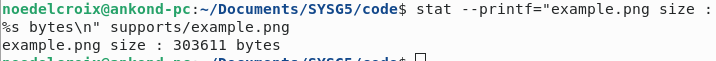
\includegraphics[width=1\textwidth]{img/lsb_size_before.png} 
Commande encodage :
\begin{lstlisting}
make build
./steganography lsb encode supports/example.png Hello World
\end{lstlisting}
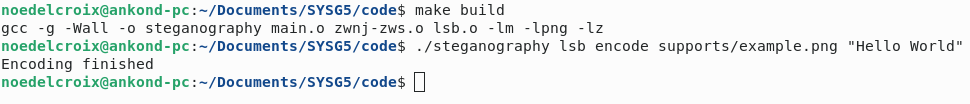
\includegraphics[width=1\textwidth]{img/lsb_encode.png} 
On check la taille de l'image après encodage :
\newline
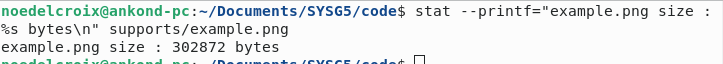
\includegraphics[width=1\textwidth]{img/lsb_size_after.png}
La donnée est bien enregistrée malgré que la taille de l'image n'est pas changée :
\newline
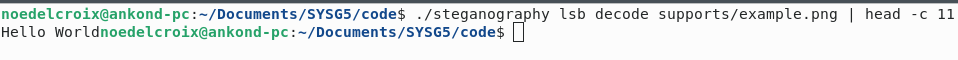
\includegraphics[width=1\textwidth]{img/lsb_decode.png}

